please note the naming pattern of source files:\\
excercise X task Y [part Z [a...z]] = \verb|eXtY[pZ[a...z].cpp|

\section{Task 1}
see \verb|e1t1p1.cpp| (using $n = 100000$; $c = 3$; $p = 31$; $x_\mathrm{seed} = 1$)

\subsection{Square test}
Correlation / square test plot: see fig \ref{fig:t1p1}
\begin{figure}[b]
  \centering
  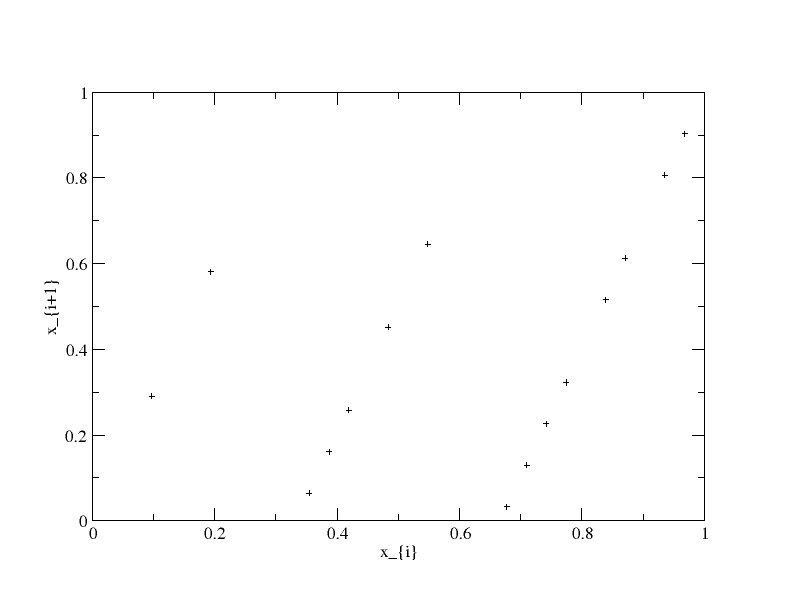
\includegraphics[width=\textwidth]{../pic/e1t1p1.png}
  \caption{Square test plot for first set of values}
  \label{fig:t1p1}
\end{figure}


\subsection{3d plot for cube test}
Cube test plot: fig. \ref{fig:cube} and \verb|e1t1p2.cpp| (using $n = 100000$; $c = 3$; $p = 31$; $x_\mathrm{seed} = 1$)

(created with matlab: \verb|plot3(rnd3d(:,1),rnd3d(:,2),rnd3d(:,3),'.')| and using gui)

\begin{figure}
  \centering
  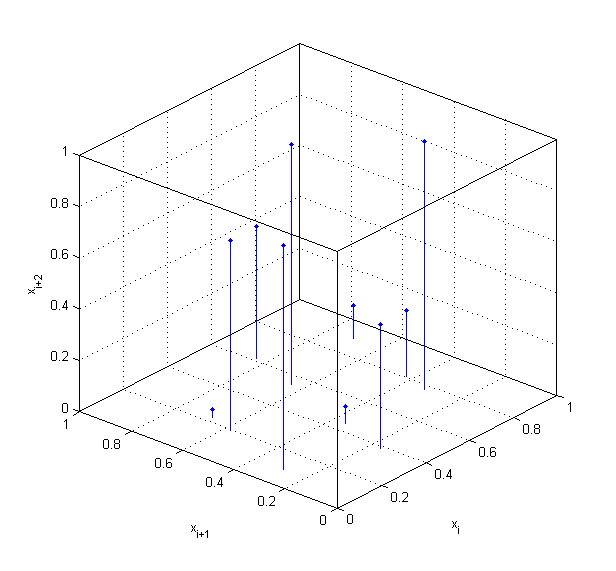
\includegraphics[width=\textwidth]{../pic/e1t1p2.png}
  \caption{Cube test plot for first set of RNG values}
  \label{fig:cube}
\end{figure}


\subsection{Other RNG's}
See \verb|e1t1p3a.cpp| for fig \ref{fig:e1t1p3a} and \verb|e1t1p3b.cpp| for fig \ref{fig:e1t1p3b} (using $n = 10000$; $c = 5648$; $p = 34875$; $x_\mathrm{seed} = 8451$)

\begin{figure}[b]
  \centering
  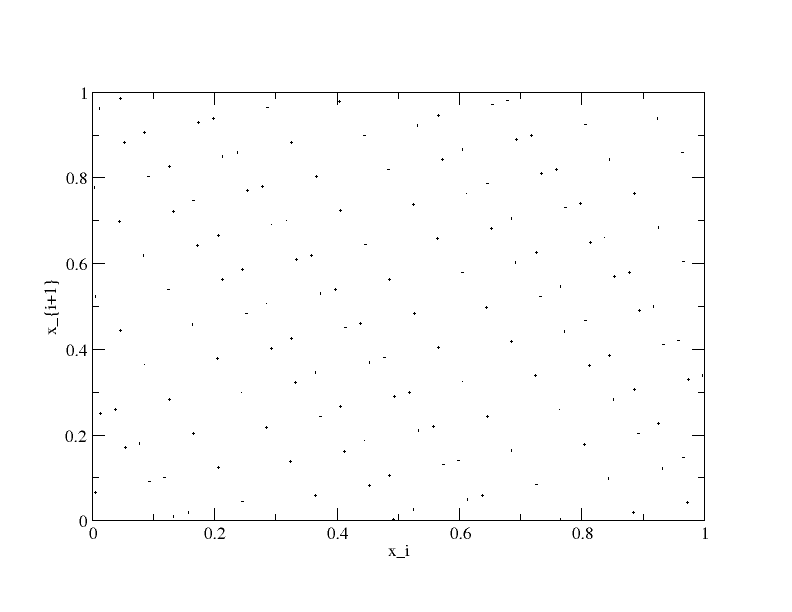
\includegraphics[width=\textwidth]{../pic/e1t1p3a.png}
  \caption{Squareplot  with second set of RNG values}
  \label{fig:e1t1p3a}
\end{figure}

\begin{figure}[b]
  \centering
  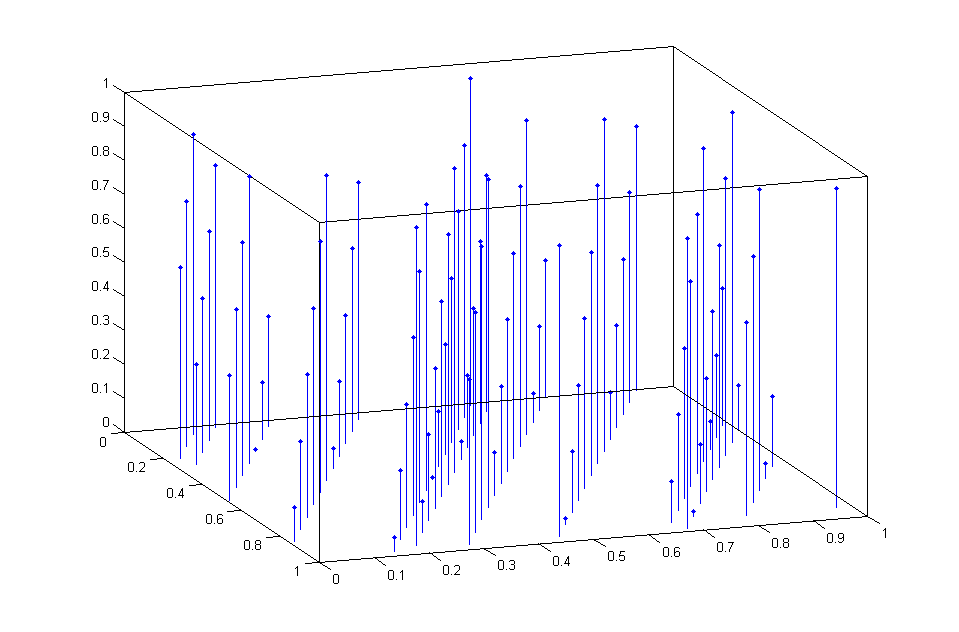
\includegraphics[width=\textwidth]{../pic/e1t1p3b.png}
  \caption{Cubeplot with second set of RNG values}
  \label{fig:e1t1p3b}
\end{figure}


\section{Task 2}
See \verb|e1t2.cpp| and plot \ref{fig:e1t2} (using $n = 10000$; $c = 16807$; $p = 2147483647$; $x_\mathrm{seed} = 1$)
Skech of idea, using cartesian coordinate system and unit circle:
\begin{itemize}
  \item generate a pair of homogeneous random points $(x_1,x_2)$, with $x_i \in [-1,1]$
  \item if $x_1^2 + x_2^2<=1$, then return the point, otherwise reject it and try again
  \item if necessairy, transform $(x_1,x_2)$ to polar coordinate system $(r,\rho)$
\end{itemize}

\begin{figure}[b]
  \centering
  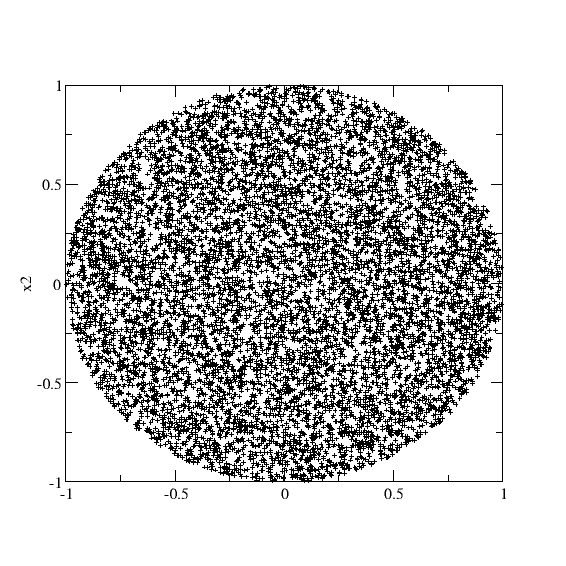
\includegraphics[width=\textwidth]{../pic/e1t2.png}
  \caption{Random numbers in a circle}
  \label{fig:e1t2}
\end{figure}


\section{Task 3}
See \verb|e1t3.cpp|, used $k=10$ bins, $n=1000$ binned random numbers ($np_i=100$).
\begin{itemize}
  \item $c = 3$; $p = 31$; $x_\mathrm{seed} = 1$: $\chi^2 = 0.1$
  \item $c = 1017$; $p = 8191$; $x_\mathrm{seed} = 154$: $\chi^2 = 5.54$
  \item built in \verb|rand()| (using init. \verb|srand(670706)|) $\chi^2 = 13.74$
\end{itemize}